\qrchapter{https://forgottenpillar.com/rsc/en-fp-chapter23}{The great apostasy is soon to be realized} \label{chap:apostasy}


\qrchapter{https://forgottenpillar.com/rsc/es-fp-chapter23}{La gran apostasía pronto se hará realidad} \label{chap:apostasy}


In 1903, when the Living Temple was published and instigated the controversy over the \emcap{personality of God}, Sister White was faithfully obeying the command of the Great Commander. She was called by the words “\textit{Meet it!}” She faced this controversy by writing numerous letters to many people in the field. In these letters, we trace the prophetic insight of the future of the Seventh-day Adventist Church.


En 1903, cuando se publicó el Living Temple e instigó la controversia sobre la \emcap{personalidad de Dios}, la hermana White estaba obedeciendo fielmente el mandato del Gran Comandante. Ella fue llamada por las palabras “\textit{¡Confrontalo!}” Ella enfrentó esta controversia escribiendo numerosas cartas a muchas personas en el campo. En estas cartas, trazamos la visión profética del futuro de la Iglesia Adventista del Séptimo Día.


One example is the correspondence between Sister White and her son William White. On November 26, 1905, there was a great Health Conference in College View Nebraska, where many medical missionary workers met together. William White was there and he had a short, 30-minute public talk. Afterwards, he wrote a letter to his mother regarding his impressions from the conference. Here is part of that letter:


Un ejemplo es la correspondencia entre la hermana White y su hijo William White. El 26 de noviembre de 1905, hubo una gran Conferencia de Salud en College View Nebraska, donde se reunieron muchos trabajadores médicos misioneros. William White estuvo allí y dio una breve charla pública de 30 minutos. Después, escribió una carta a su madre sobre sus impresiones de la conferencia. Aquí está parte de esa carta:


\others{College View, Ne. – Tuesday, November 28, 1905; Author: William C. White} \\
\others{Nov. 28, 1905.} \\
\others{Mrs. E. G. White, Sanitarium, Cala.}


\others{College View, Ne. – Martes, 28 de noviembre de 1905; Autor: William C. White} \\
\others{28 de noviembre de 1905.} \\
\others{Sra. E. G. White, Sanitarium, Cala.}


\othersnogap{...Sabbath morning I had opportunity to speak about thirty minutes. In my remarks I refered to the history of the Christian church. They began with pure principles, but through the attacks of Satan they became backslidden and departed from those principles. \textbf{I pointed out that the only hope for the S. D. A. church was to \underline{adhear to first principles}}. \textbf{I then referred to the order in which the enemy is attacking our work. His first effort was to destroy union and establish separation. His next work was to weaken our reverence for the Sabbath, then to weaken our faith in the Sanctuary service, then \underline{to break our confidence in the Spirit of Prophecy}, then to \underline{confuse our conception regarding a personal God}}.}[Letter from W. C. White to E. G. White, November 28, 1905.][http://ellenwhite.org/content/correspondence/incoming/43292pdf]


\othersnogap{...El sábado por la mañana tuve la oportunidad de hablar unos treinta minutos. En mis comentarios me referí a la historia de la iglesia cristiana. Comenzaron con principios puros, pero a través de los ataques de Satanás se volvieron reincidentes y se apartaron de esos principios. \textbf{Señalé que la única esperanza para la iglesia de los ASD era \underline{adherirse a los primeros principios}}. \textbf{Luego me referí al orden en que el enemigo está atacando nuestra obra. Su primer esfuerzo fue destruir la unión y establecer la separación. Su siguiente obra fue debilitar nuestra reverencia por el sábado, luego debilitar nuestra fe en el servicio del Santuario, luego \underline{quebrar nuestra confianza en el Espíritu de Profecía}, luego \underline{confundir nuestra concepción respecto a un Dios personal}}.}[Letter from W. C. White to E. G. White, November 28, 1905.][http://ellenwhite.org/content/correspondence/incoming/43292pdf]


\begin{figure}
    \centering
    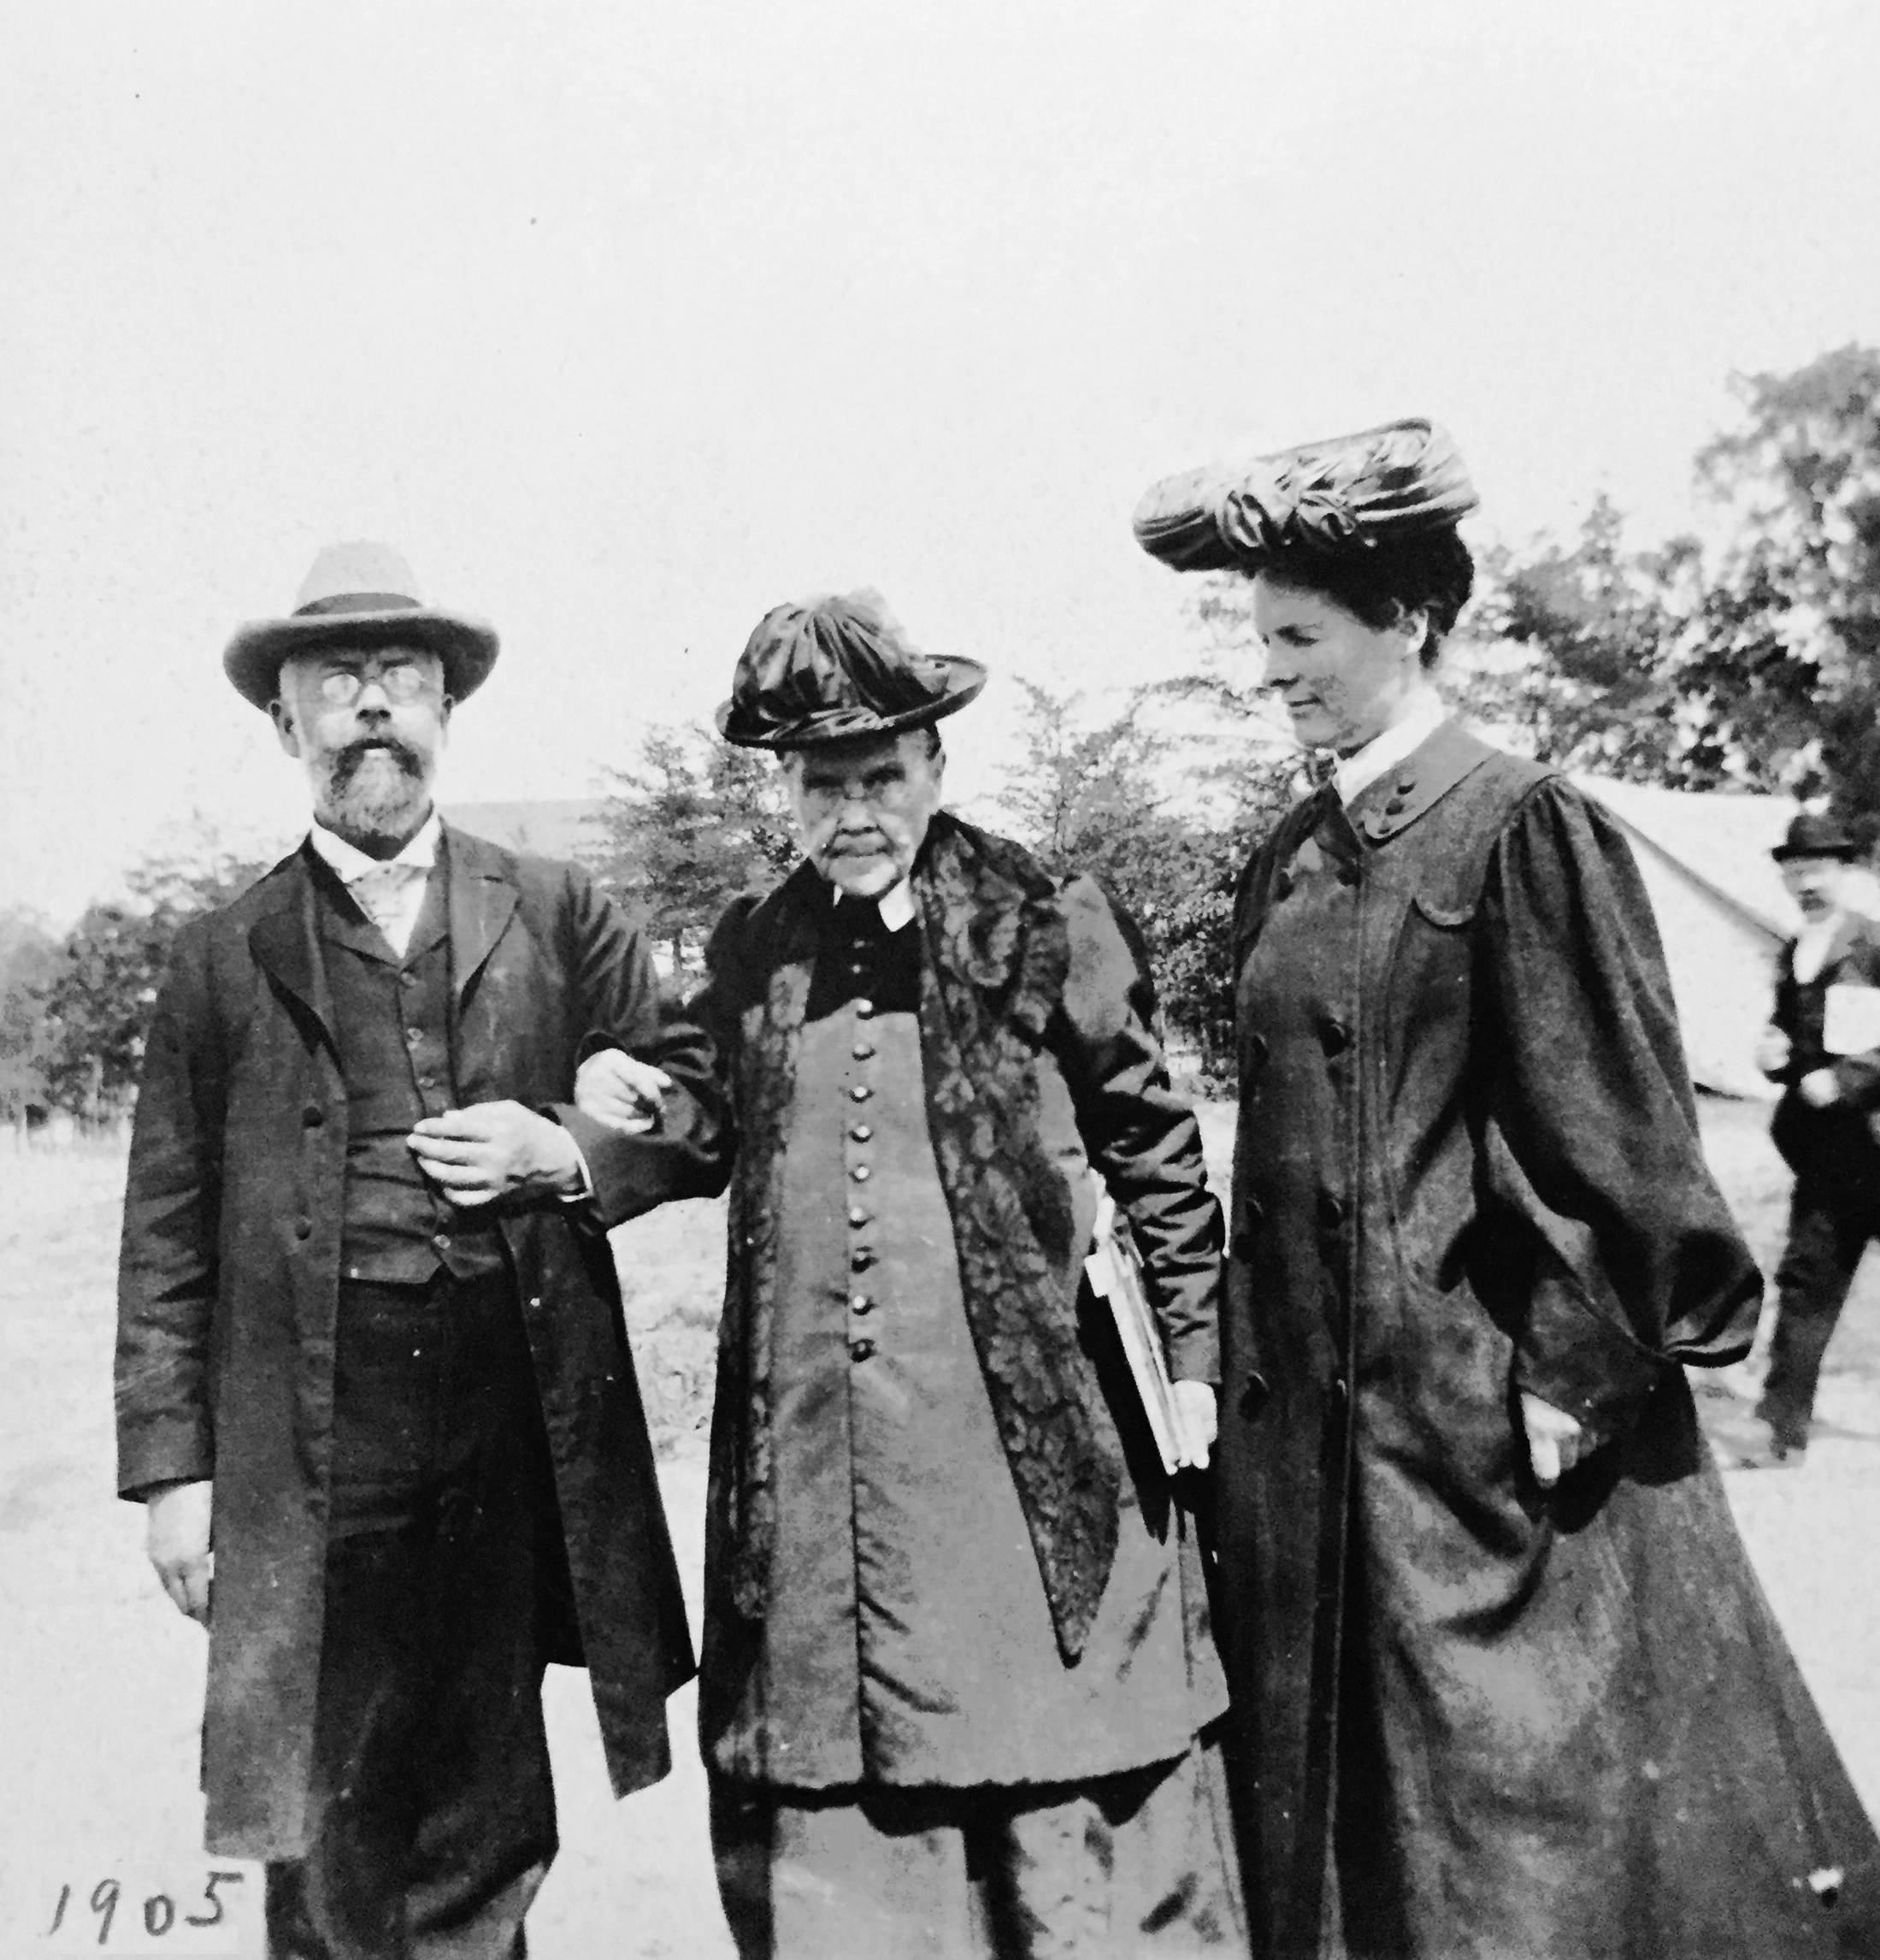
\includegraphics[width=1\linewidth]{images/william-ellen-white-1905.jpg}
    \caption*{William C. White and Ellen G. White, 1905}
    \label{fig:w-e-white}
\end{figure}


\begin{figure}
    \centering
    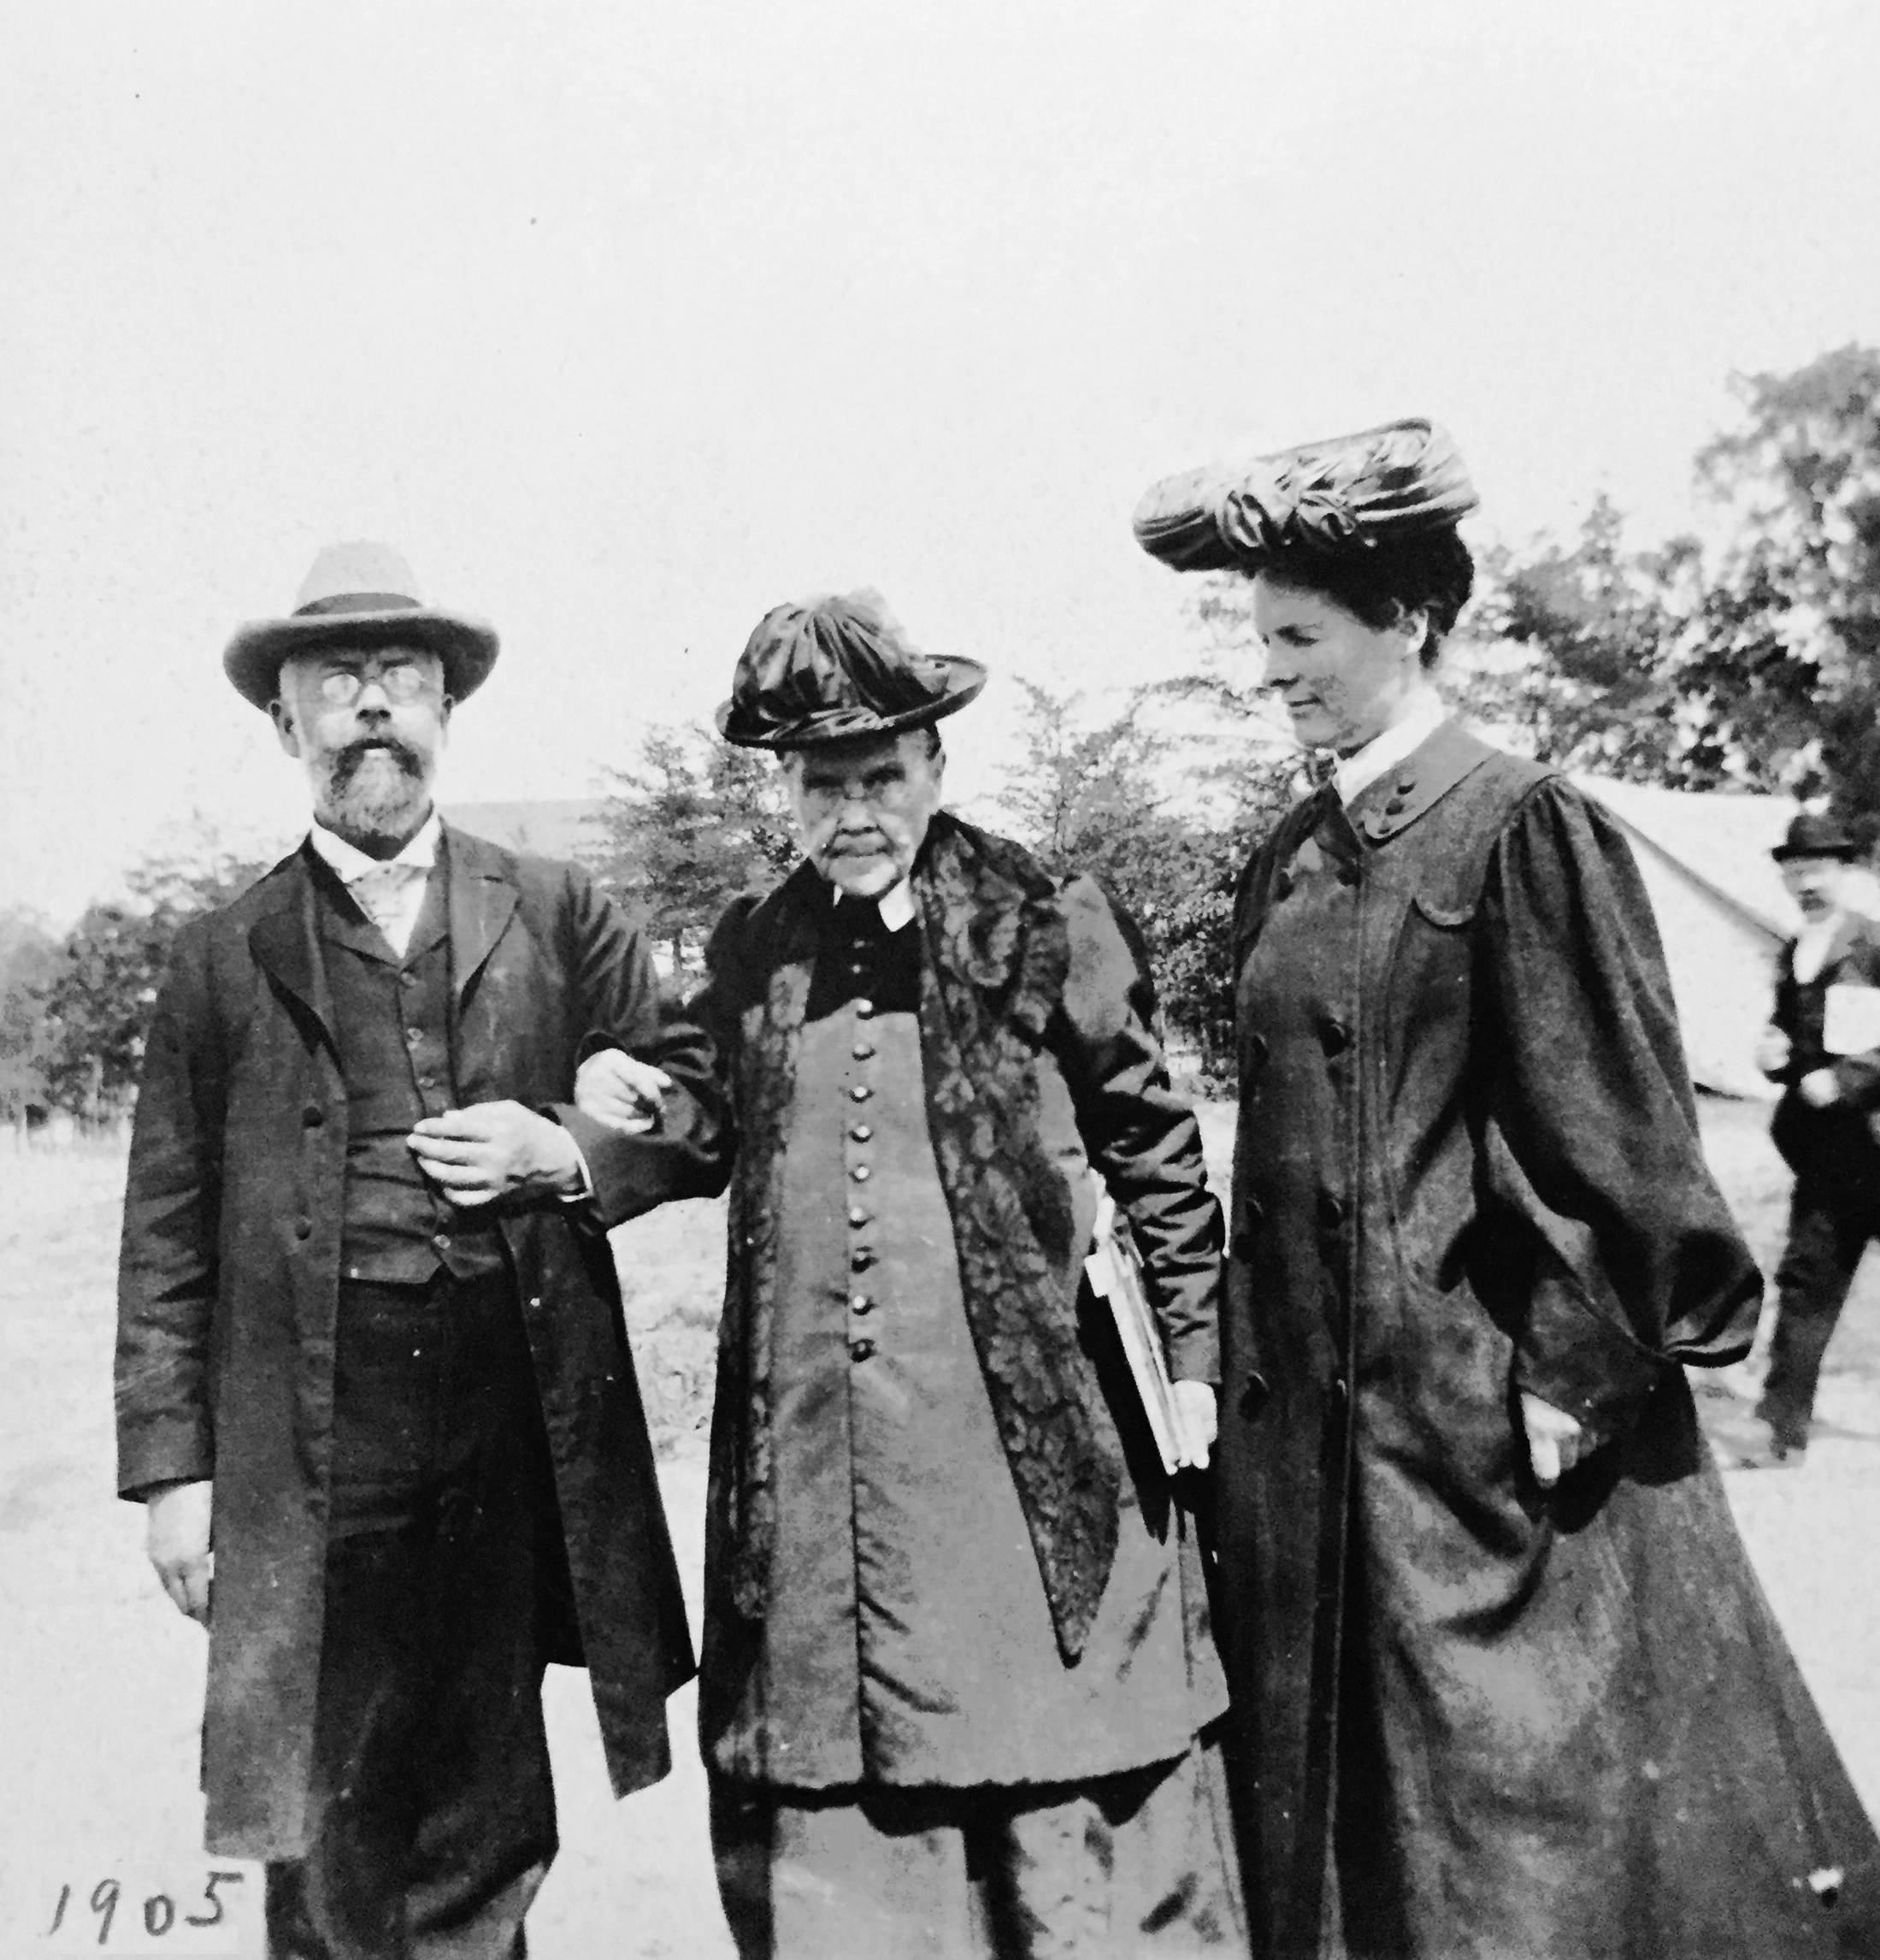
\includegraphics[width=1\linewidth]{images/william-ellen-white-1905.jpg}
    \caption*{William C. White y Ellen G. White, 1905}
    \label{fig:w-e-white}
\end{figure}


According to William White, our only hope as Seventh-day Adventists is to adhere to first principles. These principles, as we know, are the \emcap{Fundamental Principles}. Then, he referred to the order in which the enemy is attacking our work. The attack begins with our disunity, then aims to weaken our reverence for the Sabbath and the Sanctuary service, targets our confidence in the Spirit of Prophecy, and finally focuses on confusing our conceptions regarding personal God.


Según William White, nuestra única esperanza como adventistas del séptimo día es adherirnos a los primeros principios. Estos principios, como sabemos, son los \emcap{Principios Fundamentales}. Luego, se refirió al orden en que el enemigo está atacando nuestra obra. El ataque comienza con nuestra desunión, luego aspira a debilitar nuestra reverencia por el sábado y el servicio del Santuario, apunta a nuestra confianza en el Espíritu de Profecía, y finalmente se enfoca en confundir nuestras concepciones respecto al Dios personal.


Sister White’s response to William White is of a startling nature. She hints to us that the great apostasy is soon to be realized, and that our hope is to adhere to the first principles of our faith—the \emcap{Fundamental Principles}.


La respuesta de la hermana White a William White es de naturaleza sorprendente. Ella nos insinúa que la gran apostasía pronto se realizará, y que nuestra esperanza es adherirnos a los primeros principios de nuestra fe—los \emcap{Principios Fundamentales}.


\egw{Elmshaven, St. Helena, California} \\
\egw{December 4, 1905} \\
\egw{W. C. White} \\
\egw{My dear son - }


\egw{Elmshaven, St. Helena, California} \\
\egw{4 de diciembre de 1905} \\
\egw{W. C. White} \\
\egw{Mi querido hijo - }


\egw{...}


\egw{...}


\egw{“\textbf{One thing it is certain is soon to be realized—\underline{the great apostasy}, which is developing and increasing and waxing stronger and \underline{will continue} to do so until the Lord shall descend from heaven with a shout. \underline{We are to hold fast the first principles of our denominated faith} and go forward from strength to increased faith. \underline{Ever} we are to keep the faith that has been substantiated by the Holy Spirit of God \underline{from the earlier events of our experience until the present time}.} We need now larger breadth and deeper, more earnest, unwavering faith in the leadings of the Holy Spirit. \textbf{If we needed the manifest proof of the Holy Spirit’s power to confirm truth \underline{in the beginning}, after the passing of the time, \underline{we need today all the evidence in the confirmation of the truth}, when souls are departing from the faith and giving heed to seducing spirits and doctrines of devils.} There must not be any languishing of soul now. If ever there was a period of time when we needed the Holy Spirit’s power in our discourses, in our prayers, in every action proposed, it is now. \textbf{We are not to stop at the first experience, but while we bear \underline{the same message} to the people, \underline{this message is to be strengthened and enlarged}}. \textbf{We are to see and realize the importance of the message made certain by its divine origin}. We are to follow on to know the Lord, that we may know that His going forth is prepared as the morning. Our souls need the quickening from the Source of all power. \textbf{We may be strengthened and confirmed in the past experience \underline{that holds us to the essential points of truth which have made us what we are—Seventh-day Adventists}.}“}[Lt326-1905.2; 1905][https://egwwritings.org/read?panels=p7678.8]


\egw{“\textbf{Una cosa es segura que pronto se realizará—\underline{la gran apostasía}, que se está desarrollando y aumentando y se hace más fuerte y \underline{continuará} haciéndolo hasta que el Señor descienda del cielo con un grito. \underline{Debemos mantener firmes los primeros principios de nuestra denominada fe} y avanzar con fuerza hacia una fe mayor. \underline{Siempre} hemos de mantener la fe que ha sido corroborada por el Espíritu Santo de Dios \underline{desde los primeros acontecimientos de nuestra experiencia hasta el momento presente}.} Ahora necesitamos una mayor amplitud y una fe más profunda, sincera e inquebrantable en la dirección del Espíritu Santo. \textbf{Si necesitábamos la prueba manifiesta del poder del Espíritu Santo para confirmar la verdad \underline{en el principio}, después del paso del tiempo, \underline{necesitamos hoy toda la evidencia en la confirmación de la verdad}, cuando las almas se están apartando de la fe y prestando atención a los espíritus seductores y a las doctrinas de los demonios.} No debe haber ahora ninguna languidez del alma. Si alguna vez hubo un período de tiempo en que necesitamos el poder del Espíritu Santo en nuestros discursos, en nuestras oraciones, en cada acción propuesta, es ahora. \textbf{No hemos de detenernos en la primera experiencia, sino que, mientras llevemos \underline{el mismo mensaje} al pueblo, \underline{este mensaje ha de ser reforzado y ampliado}}. \textbf{Hemos de ver y comprender la importancia del mensaje que se ha hecho cierto por su origen divino}. Hemos de seguir para conocer al Señor, para saber que su salida está preparada como la mañana. Nuestras almas necesitan la vivificación de la Fuente de todo poder. \textbf{Podemos ser fortalecidos y confirmados en la experiencia pasada \underline{que nos mantiene en los puntos esenciales de la verdad que nos han hecho lo que somos—Adventistas del Séptimo Día}.}”}[Lt326-1905.2; 1905][https://egwwritings.org/read?panels=p7678.8]


\egwnogap{\textbf{The past fifty years have not dimmed one jot or principle of our faith as we received the great and wonderful evidences that were made certain to us in 1844, after the passing of the time.} The languishing souls are to be confirmed and quickened according to His Word. And many of the ministers of the gospel and the Lord’s physicians will have their languishing souls quickened according to the Word. \textbf{\underline{Not a word is changed or denied}.} \textbf{That which the Holy Spirit testified to as truth after the passing of the time, in our great disappointment, is \underline{the solid foundation of truth}. Pillars of truth were revealed, and we accepted \underline{the foundation principles} that have made us what we are—Seventh-day Adventists, keeping the commandments of God and having the faith of Jesus.}}[Lt326-1905.3; 1905][https://egwwritings.org/read?panels=p7678.9]


\egwnogap{\textbf{Los últimos cincuenta años no han atenuado ni una jota ni un principio de nuestra fe al recibir las grandes y maravillosas evidencias que se nos hicieron ciertas en 1844, después del paso del tiempo.} Las almas que languidecen han de ser confirmadas y vivificadas según Su Palabra. Y muchos de los ministros del evangelio y los médicos del Señor tendrán sus almas languidecientes vivificadas de acuerdo con la Palabra. \textbf{\underline{Ni una palabra es cambiada o negada}.} \textbf{Lo que el Espíritu Santo testificó como verdad después del paso del tiempo, en nuestra gran decepción, es \underline{el sólido fundamento de la verdad}. Se revelaron los pilares de la verdad, y aceptamos \underline{los principios fundamentales} que nos han convertido en lo que somos—Adventistas del Séptimo Día, guardando los mandamientos de Dios y teniendo la fe de Jesús.}}[Lt326-1905.3; 1905][https://egwwritings.org/read?panels=p7678.9]


This letter is startling because it is an answer to the order of how the enemy is attacking our work. Sister White is well aware of these attacks and she presented the problem in its correct light, also showing us what we shall do to prevent Satan's attacks on us. The enemy wants to \others{confuse our conception regarding a personal God}. This is the very point of great apostasy that \egwinline{is soon to be realized}, and has been \egwinline{developing and increasing and waxing stronger and will continue to do so until the Lord shall descend from heaven with a shout}. This is the apostasy we are experiencing today. What is our hope against this deception and great apostasy? \egwinline{\textbf{\underline{We are to hold fast the first principles of our denominated faith} and go forward from strength to increased faith. \underline{Ever} we are to keep the faith that has been substantiated by the Holy Spirit of God from the earlier events of our experience until the present time.}} \egwinline{...\textbf{\underline{this message is to be strengthened and enlarged}}...} \egwinline{...\textbf{\underline{we need today all the evidence in the confirmation of the truth}}...} \egwinline{\textbf{We may be strengthened and confirmed in the past experience that holds us to the essential points of truth which have made us what we are—Seventh-day Adventists}}. These essential points of truth, which have made us Seventh-day Adventists, are the \emcap{Fundamental Principles}, born in the beginning of our work. In 1905, she wrote, \egwinline{\textbf{The past fifty years have not dimmed one jot or principle of our faith as we received the great and wonderful evidences that were made certain to us in 1844, after the passing of the time.}} \egwinline{\textbf{Not a word is changed or denied.} \textbf{That which the Holy Spirit testified to as truth after the passing of the time, in our great disappointment, is \underline{the solid foundation of truth}. Pillars of truth were revealed, and we accepted \underline{the foundation principles} that have made us what we are—Seventh-day Adventists, keeping the commandments of God and having the faith of Jesus.}}


Esta carta es sorprendente porque es una respuesta a la orden de cómo el enemigo está atacando nuestra obra. La hermana White está muy consciente de estos ataques y presentó el problema en su luz correcta, mostrándonos también lo que debemos hacer para prevenir los ataques de Satanás contra nosotros. El enemigo quiere \others{confundir nuestra concepción respecto a un Dios personal}. Este es el punto de la gran apostasía que \egwinline{pronto se realizará}, y ha estado \egwinline{desarrollándo y aumentando y se hace más fuerte y continuará haciéndolo hasta que el Señor descienda del cielo con un grito}. Esta es la apostasía que estamos viviendo hoy. ¿Cuál es nuestra esperanza contra este engaño y gran apostasía? \egwinline{\textbf{\underline{Debemos mantener firmes los primeros principios de nuestra denominada fe} y avanzar con fuerza hacia una fe mayor. \underline{Siempre} hemos de mantener la fe que ha sido corroborada por el Espíritu Santo de Dios desde los primeros acontecimientos de nuestra experiencia hasta el momento presente.}} \egwinline{...\textbf{\underline{este mensaje ha de ser reforzado y ampliado}}...} \egwinline{...\textbf{\underline{necesitamos hoy toda la evidencia en la confirmación de la verdad}}...} \egwinline{\textbf{Podemos ser fortalecidos y confirmados en la experiencia pasada que nos mantiene en los puntos esenciales de la verdad que nos han hecho lo que somos—Adventistas del Séptimo Día}}. Estos puntos esenciales de la verdad, que nos han hecho adventistas del séptimo día, son los \emcap{Principios Fundamentales}, nacidos en el comienzo de nuestra obra. En 1905, escribió, \egwinline{\textbf{Los últimos cincuenta años no han atenuado ni una jota ni un principio de nuestra fe al recibir las grandes y maravillosas evidencias que se nos hicieron ciertas en 1844, después del paso del tiempo.}} \egwinline{\textbf{Ni una palabra es cambiada o negada.} \textbf{Lo que el Espíritu Santo testificó como verdad después del paso del tiempo, en nuestra gran decepción, es \underline{el sólido fundamento de la verdad}. Se revelaron los pilares de la verdad, y aceptamos \underline{los principios fundamentales} que nos han convertido en lo que somos—Adventistas del Séptimo Día, guardando los mandamientos de Dios y teniendo la fe de Jesús.}}


God calls us to be steadfast in the \emcap{Fundamental Principles}, especially over the \others{conception regarding a personal God}. This is the first point of the \emcap{Fundamental Principles}.


Dios nos llama a ser firmes en los \emcap{Principios Fundamentales}, especialmente sobre la \others{concepción respecto a un Dios personal}. Este es el primer punto de los \emcap{Principios Fundamentales}.


Sister White foretold that a great apostasy is developing in our church regarding the understanding of the \emcap{personality of God}. The true understanding of the \emcap{personality of God} is presented in the \emcap{Fundamental Principles}. She clearly warned us of Satan’s attack on these principles. She calls us to \egw{\textbf{hold fast the first principles of our denominated faith} and go forward from strength to increased faith}.


La hermana White predijo que se está desarrollando una gran apostasía en nuestra iglesia con respecto a la comprensión de la \emcap{personalidad de Dios}. La verdadera comprensión de la \emcap{personalidad de Dios} se presenta en los \emcap{Principios Fundamentales}. Ella nos advirtió claramente del ataque de Satanás a estos principios. Ella nos llama a \egw{\textbf{mantener firmes los primeros principios de nuestra denominada fe} y avanzar con fuerza hacia una fe mayor}.


\egw{\textbf{“After the passing of the time, God entrusted to His faithful followers the precious \underline{principles of present truth}. These principles were not given to those who had had no part in the giving of the first and second angels’ messages. They were given to the workers who had had a part in the cause from the beginning}.”}[Ms129-1905.5; 1905][https://egwwritings.org/read?panels=p9797.12]


\egw{\textbf{“Después del paso del tiempo, Dios confió a sus fieles seguidores los preciosos \underline{principios de la verdad presente}. Estos principios no fueron dados a los que no habían tenido parte en la entrega de los mensajes del primer y segundo ángeles. Fueron dados a los obreros que habían tenido parte en la causa desde el principio}.”}[Ms129-1905.5; 1905][https://egwwritings.org/read?panels=p9797.12]


\egwnogap{\textbf{Those who passed through these experiences are to be as \underline{firm as a rock to the principles} that have made us Seventh-day Adventists}. They are to be workers together with God, binding up the testimony and sealing the law among His disciples. Those who took part in the establishment of our work upon the foundation of Bible truth; \textbf{those who know the waymarks that have pointed out the right path} are to be regarded as workers of the highest value. They can speak from personal experience, regarding the truths entrusted to them. These men are not to permit their faith to be changed to infidelity; they are not to permit the banner of the third angel to be taken from their hands. They are to hold the beginning of their confidence firm unto the end. \textbf{\underline{The Lord has declared that the history of the past shall be rehearsed as we enter upon the closing work}. Every truth that He has given for these last days is to be proclaimed to the world. \underline{Every pillar} that He has established \underline{is to be strengthened}. We cannot now step off the foundation that God has established. We cannot now enter into any new organization; for this would mean apostasy from the truth}.}[Ms129-1905.6; 1905][https://egwwritings.org/read?panels=p9797.13]


\egwnogap{\textbf{Los que pasaron por estas experiencias han de ser tan \underline{firmes como una roca en los principios} que nos han hecho adventistas del séptimo día}. Deben ser obreros juntos con Dios, atando el testimonio y sellando la ley entre sus discípulos. Los que participaron en el establecimiento de nuestra obra sobre el fundamento de la verdad bíblica; \textbf{los que conocen los hitos que han señalado el camino correcto} deben ser considerados como obreros del más alto valor. Pueden hablar por experiencia personal, respecto a las verdades que se les han confiado. Estos hombres no deben permitir que su fe sea cambiada por la infidelidad; no deben permitir que el estandarte del tercer ángel sea arrebatado de sus manos. Deben mantener firme el principio de su confianza hasta el final. \textbf{\underline{El Señor ha declarado que la historia del pasado será ensayada al entrar en la obra final}. Cada verdad que Él ha dado para estos últimos días debe ser proclamada al mundo. \underline{Cada pilar} que Él ha establecido \underline{debe ser fortalecido}. No podemos ahora salirnos del fundamento que Dios ha establecido. No podemos ahora entrar en ninguna nueva organización; porque esto significaría apostasía de la verdad}.}[Ms129-1905.6; 1905][https://egwwritings.org/read?panels=p9797.13]


Stepping off of the foundation that God has established means entering into new organization; this is apostasy from the truth. Comparing the \emcap{Fundamental Principles} of the past with current trinitarian Fundamental Beliefs, it’s evident we’re in a state of apostasy.  Ellen White prophesied that this apostasy will be \egwinline{\textbf{developing and increasing and waxing stronger and \underline{will continue} to do so until the Lord shall descend from heaven with a shout}}[Lt326-1905.2; 1905][https://egwwritings.org/read?panels=p7678.8].


Salirse del fundamento que Dios ha establecido significa entrar en una nueva organización; esto es apostasía de la verdad. Al comparar los \emcap{Principios Fundamentales} del pasado con las creencias fundamentales trinitarias actuales, es evidente que estamos en un estado de apostasía. Elena G. de White profetizó que esta apostasía se \egwinline{\textbf{desarrollará y aumentará y se hará más fuerte y \underline{continuará} haciéndolo hasta que el Señor descienda del cielo con un grito}}[Lt326-1905.2; 1905][https://egwwritings.org/read?panels=p7678.8].


% The great apostasy is soon to be realized

\begin{titledpoem}
    
    \stanza{
        In a letter penned, a crisis foretold, \\
        From Ellen White, a warning bold: \\
        "Adhere to the roots of our Adventist comprehend, \\
        For soon will come apostasy's seed."
    }

    \stanza{
        The pillars strong of our founding year, \\
        Are under siege, as Ellen feared. \\
        To "Meet it!" was her stern command, \\
        To hold the line, to firmly stand.
    }

    \stanza{
        "Keep to the principles," her urgent plea, \\
        From 1844's prophetic decree. \\
        For truth confirmed by the Spirit's flame, \\
        Shall not be denied, nor put to shame.
    }

    \stanza{
        The enemy seeks to divide and sway, \\
        To change our course, to lead astray. \\
        But steadfast hearts must ever cling \\
        To the first truths that made our spirits sing.
    }

    \stanza{
        Hold fast, she wrote, to what we know, \\
        The Fundamental Principles that show \\
        The way to live, the path to trod, \\
        Under the gaze of an unchanging God.
    }

    \stanza{
        For as the world spins toward its close, \\
        The truth of Ellen White still glows— \\
        A beacon strong against the night, \\
        Guiding the faithful in the right.
    }
    
\end{titledpoem}


% \chapter{The great apostasy is soon to be realized} \label{chap:apostasy}

In 1903, when the Living Temple was published and instigated the controversy over the \emcap{personality of God}, Sister White was faithfully obeying the command of the Great Commander. She was called by the words “\textit{Meet it!}” She faced this controversy by writing numerous letters to many people in the field. In these letters, we trace the prophetic insight of the future of the Seventh-day Adventist Church.

One example is the correspondence between Sister White and her son William White. On November 26, 1905, there was a great Health Conference in College View Nebraska, where many medical missionary workers met together. William White was there and he had a short, 30-minute public talk. Afterwards, he wrote a letter to his mother regarding his impressions from the conference. Here is part of that letter: 

\others{College View, Ne. – Tuesday, November 28, 1905; Author: William C. White} \\
\others{Nov. 28, 1905.} \\
\others{Mrs. E. G. White, Sanitarium, Cala.}

\othersnogap{...Sabbath morning I had opportunity to speak about thirty minutes. In my remarks I refered to the history of the Christian church. They began with pure principles, but through the attacks of Satan they became backslidden and departed from those principles. \textbf{I pointed out that the only hope for the S. D. A. church was to \underline{adhear to first principles}}. \textbf{I then referred to the order in which the enemy is attacking our work. His first effort was to destroy union and establish separation. His next work was to weaken our reverence for the Sabbath, then to weaken our faith in the Sanctuary service, then \underline{to break our confidence in the Spirit of Prophecy}, then to \underline{confuse our conception regarding a personal God}}.}[Letter from W. C. White to E. G. White, November 28, 1905.][http://ellenwhite.org/content/correspondence/incoming/43292pdf]

\begin{figure}
    \centering
    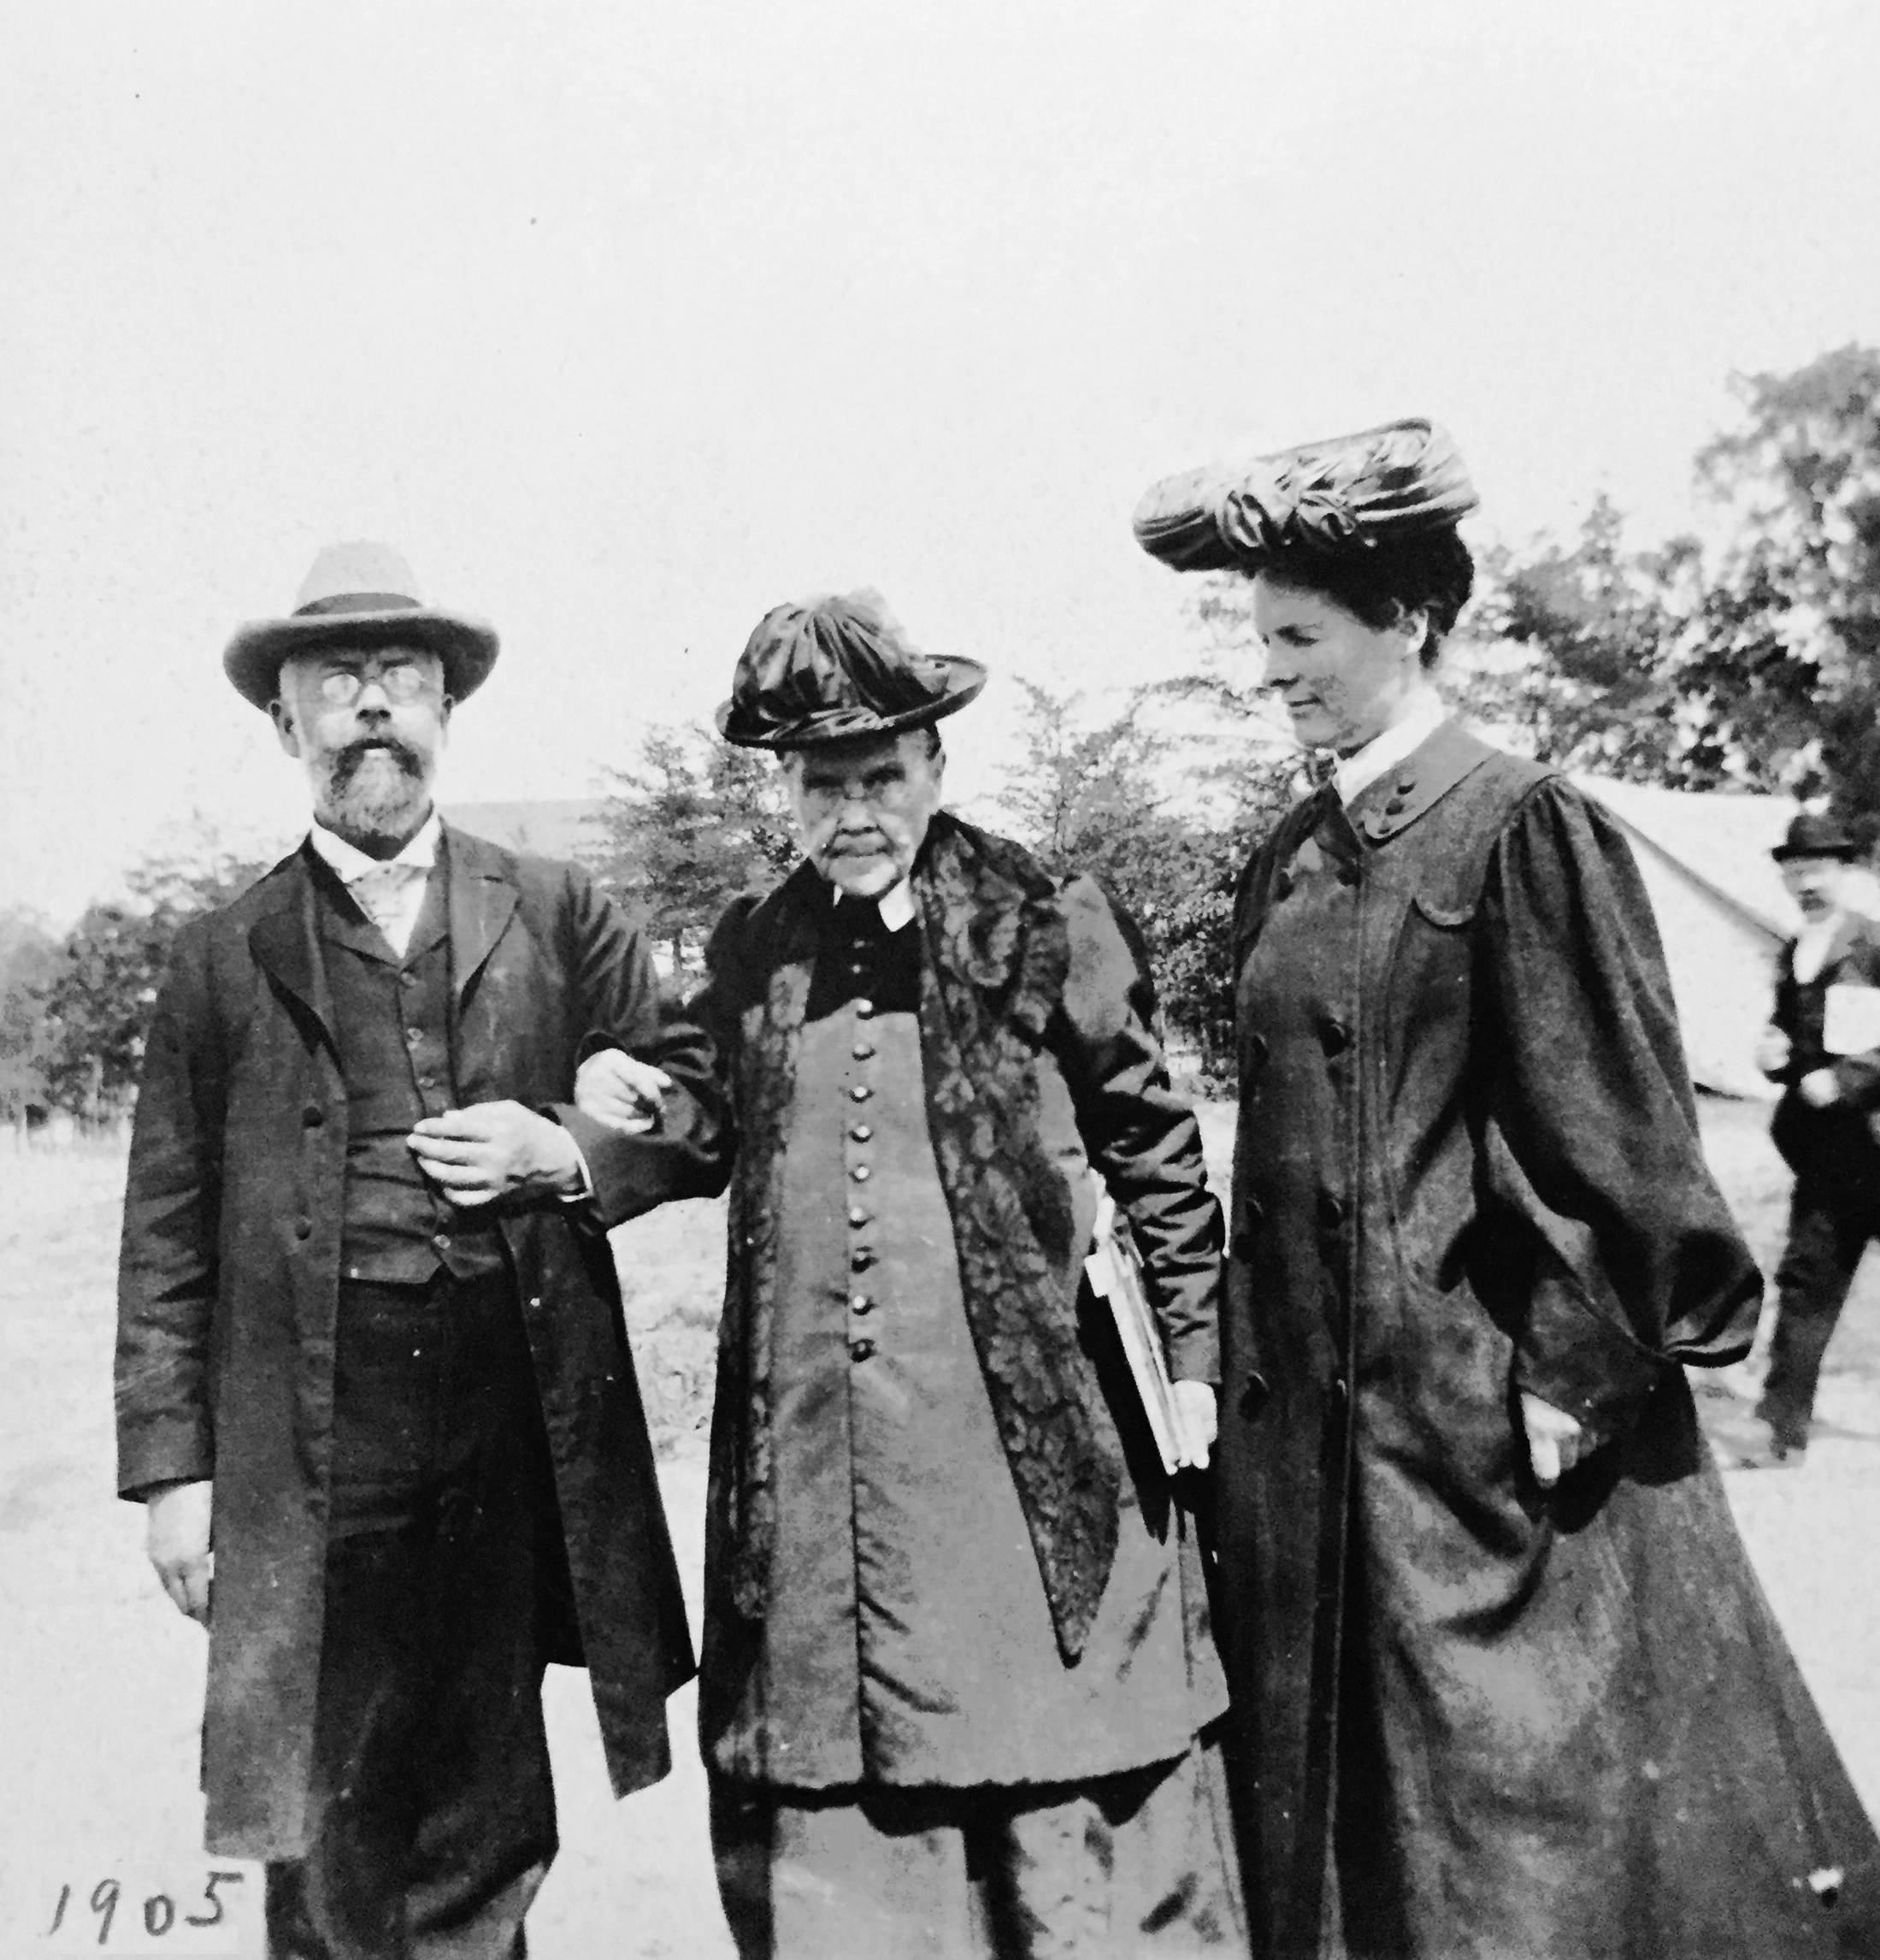
\includegraphics[width=1\linewidth]{images/william-ellen-white-1905.jpg}
    \caption*{William C. White and Ellen G. White, 1905}
    \label{fig:w-e-white}
\end{figure}

According to William White, our only hope as Seventh-day Adventists is to adhere to first principles. These principles, as we know, are the \emcap{Fundamental Principles}. Then, he referred to the order in which the enemy is attacking our work. The attack begins with our disunity, then aims to weaken our reverence for the Sabbath and the Sanctuary service, targets our confidence in the Spirit of Prophecy, and finally focuses on confusing our conceptions regarding personal God.

Sister White’s response to William White is of a startling nature. She hints to us that the great apostasy is soon to be realized, and that our hope is to adhere to the first principles of our faith—the \emcap{Fundamental Principles}.

\egw{Elmshaven, St. Helena, California} \\
\egw{December 4, 1905} \\
\egw{W. C. White} \\
\egw{My dear son - }

\egw{...}

\egw{“\textbf{One thing it is certain is soon to be realized—\underline{the great apostasy}, which is developing and increasing and waxing stronger and \underline{will continue} to do so until the Lord shall descend from heaven with a shout. \underline{We are to hold fast the first principles of our denominated faith} and go forward from strength to increased faith. \underline{Ever} we are to keep the faith that has been substantiated by the Holy Spirit of God \underline{from the earlier events of our experience until the present time}.} We need now larger breadth and deeper, more earnest, unwavering faith in the leadings of the Holy Spirit. \textbf{If we needed the manifest proof of the Holy Spirit’s power to confirm truth \underline{in the beginning}, after the passing of the time, \underline{we need today all the evidence in the confirmation of the truth}, when souls are departing from the faith and giving heed to seducing spirits and doctrines of devils.} There must not be any languishing of soul now. If ever there was a period of time when we needed the Holy Spirit’s power in our discourses, in our prayers, in every action proposed, it is now. \textbf{We are not to stop at the first experience, but while we bear \underline{the same message} to the people, \underline{this message is to be strengthened and enlarged}}. \textbf{We are to see and realize the importance of the message made certain by its divine origin}. We are to follow on to know the Lord, that we may know that His going forth is prepared as the morning. Our souls need the quickening from the Source of all power. \textbf{We may be strengthened and confirmed in the past experience \underline{that holds us to the essential points of truth which have made us what we are—Seventh-day Adventists}.}“}[Lt326-1905.2; 1905][https://egwwritings.org/read?panels=p7678.8]

\egwnogap{\textbf{The past fifty years have not dimmed one jot or principle of our faith as we received the great and wonderful evidences that were made certain to us in 1844, after the passing of the time.} The languishing souls are to be confirmed and quickened according to His Word. And many of the ministers of the gospel and the Lord’s physicians will have their languishing souls quickened according to the Word. \textbf{\underline{Not a word is changed or denied}.} \textbf{That which the Holy Spirit testified to as truth after the passing of the time, in our great disappointment, is \underline{the solid foundation of truth}. Pillars of truth were revealed, and we accepted \underline{the foundation principles} that have made us what we are—Seventh-day Adventists, keeping the commandments of God and having the faith of Jesus.}}[Lt326-1905.3; 1905][https://egwwritings.org/read?panels=p7678.9]

This letter is startling because it is an answer to the order of how the enemy is attacking our work. Sister White is well aware of these attacks and she presented the problem in its correct light, also showing us what we shall do to prevent Satan's attacks on us. The enemy wants to \others{confuse our conception regarding a personal God}. This is the very point of great apostasy that \egwinline{is soon to be realized}, and has been \egwinline{developing and increasing and waxing stronger and will continue to do so until the Lord shall descend from heaven with a shout}. This is the apostasy we are experiencing today. What is our hope against this deception and great apostasy? \egwinline{\textbf{\underline{We are to hold fast the first principles of our denominated faith} and go forward from strength to increased faith. \underline{Ever} we are to keep the faith that has been substantiated by the Holy Spirit of God from the earlier events of our experience until the present time.}} \egwinline{...\textbf{\underline{this message is to be strengthened and enlarged}}...} \egwinline{...\textbf{\underline{we need today all the evidence in the confirmation of the truth}}...} \egwinline{\textbf{We may be strengthened and confirmed in the past experience that holds us to the essential points of truth which have made us what we are—Seventh-day Adventists}}. These essential points of truth, which have made us Seventh-day Adventists, are the \emcap{Fundamental Principles}, born in the beginning of our work. In 1905, she wrote, \egwinline{\textbf{The past fifty years have not dimmed one jot or principle of our faith as we received the great and wonderful evidences that were made certain to us in 1844, after the passing of the time.}} \egwinline{\textbf{Not a word is changed or denied.} \textbf{That which the Holy Spirit testified to as truth after the passing of the time, in our great disappointment, is \underline{the solid foundation of truth}. Pillars of truth were revealed, and we accepted \underline{the foundation principles} that have made us what we are—Seventh-day Adventists, keeping the commandments of God and having the faith of Jesus.}}

God calls us to be steadfast in the \emcap{Fundamental Principles}, especially over the \others{conception regarding a personal God}. This is the first point of the \emcap{Fundamental Principles}.

Sister White foretold that a great apostasy is developing in our church regarding the understanding of the \emcap{personality of God}. The true understanding of the \emcap{personality of God} is presented in the \emcap{Fundamental Principles}. She clearly warned us of Satan’s attack on these principles. She calls us to \egw{\textbf{hold fast the first principles of our denominated faith} and go forward from strength to increased faith}.

\egw{\textbf{“After the passing of the time, God entrusted to His faithful followers the precious \underline{principles of present truth}. These principles were not given to those who had had no part in the giving of the first and second angels’ messages. They were given to the workers who had had a part in the cause from the beginning}.”}[Ms129-1905.5; 1905][https://egwwritings.org/read?panels=p9797.12]

\egwnogap{\textbf{Those who passed through these experiences are to be as \underline{firm as a rock to the principles} that have made us Seventh-day Adventists}. They are to be workers together with God, binding up the testimony and sealing the law among His disciples. Those who took part in the establishment of our work upon the foundation of Bible truth; \textbf{those who know the waymarks that have pointed out the right path} are to be regarded as workers of the highest value. They can speak from personal experience, regarding the truths entrusted to them. These men are not to permit their faith to be changed to infidelity; they are not to permit the banner of the third angel to be taken from their hands. They are to hold the beginning of their confidence firm unto the end. \textbf{\underline{The Lord has declared that the history of the past shall be rehearsed as we enter upon the closing work}. Every truth that He has given for these last days is to be proclaimed to the world. \underline{Every pillar} that He has established \underline{is to be strengthened}. We cannot now step off the foundation that God has established. We cannot now enter into any new organization; for this would mean apostasy from the truth}.}[Ms129-1905.6; 1905][https://egwwritings.org/read?panels=p9797.13]

Stepping off of the foundation that God has established means entering into new organization; this is apostasy from the truth. Comparing the \emcap{Fundamental Principles} of the past with current trinitarian Fundamental Beliefs, it’s evident we’re in a state of apostasy.  Ellen White prophesied that this apostasy will be \egwinline{\textbf{developing and increasing and waxing stronger and \underline{will continue} to do so until the Lord shall descend from heaven with a shout}}[Lt326-1905.2; 1905][https://egwwritings.org/read?panels=p7678.8].

% The great apostasy is soon to be realized

\begin{titledpoem}
    
    \stanza{
        In a letter penned, a crisis foretold, \\
        From Ellen White, a warning bold: \\
        "Adhere to the roots of our Adventist comprehend, \\
        For soon will come apostasy's seed."
    }

    \stanza{
        The pillars strong of our founding year, \\
        Are under siege, as Ellen feared. \\
        To "Meet it!" was her stern command, \\
        To hold the line, to firmly stand.
    }

    \stanza{
        "Keep to the principles," her urgent plea, \\
        From 1844's prophetic decree. \\
        For truth confirmed by the Spirit's flame, \\
        Shall not be denied, nor put to shame.
    }

    \stanza{
        The enemy seeks to divide and sway, \\
        To change our course, to lead astray. \\
        But steadfast hearts must ever cling \\
        To the first truths that made our spirits sing.
    }

    \stanza{
        Hold fast, she wrote, to what we know, \\
        The Fundamental Principles that show \\
        The way to live, the path to trod, \\
        Under the gaze of an unchanging God.
    }

    \stanza{
        For as the world spins toward its close, \\
        The truth of Ellen White still glows— \\
        A beacon strong against the night, \\
        Guiding the faithful in the right.
    }
    
\end{titledpoem}
